\rhead{7. Dijagrami aktivnosti}
\section{Dijagrami aktivnosti}
\par U nastavku se nalaze dijagrami aktivnosti korišćeni za analizu zahteva i specifikaciju dizajna.
Opisana su 4 dijagrama aktivnosti:
\begin{enumerate}
    \item \textbf{Aktivnost objave}
    \item todo
    \item todo
    \item todo
\end{enumerate}
\subsection{Aktivnost objave}
\par Dijagram aktivnosti objave predstavlja proces kojim \textit{član} kreira objavu, a \textit{volonter} je prihvata ili odbija.
Prikazana je pomoću dva dijagrama aktivnosti: kreiranje objave [Slika \ref{fig:activity-create-post}] i pregled objave [Slika \ref{fig:activity-post-review}].
\subsubsection*{Aktivnost kreiranja objave}
\par Nakon prijave, članu se nudi mogućnost da otvori formu za objavu. U formu se unose potrebne informacije o životinji u vidu teksta, slike ili videa.
Sva polja moraju biti popunjena, u suprotnom se članu prikazuje poruka greške. Nakon uspešne provere unesenih podataka, korsnik se obaveštava da je 
objava uspešno kreirana. Ovo je prikazano na slici \ref{fig:activity-create-post}.
\begin{figure}[h]
    \centering
    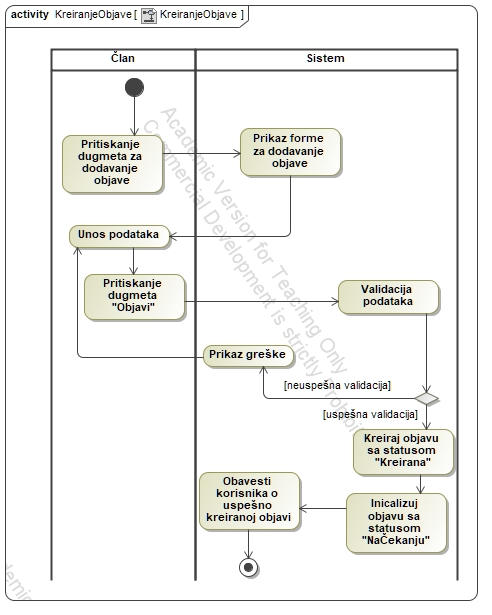
\includegraphics[width=\textwidth, height=0.75\textwidth]{img/activity-create-post.jpg}
    \caption{Dijagram aktivnosti za kreiranje objave}
    \label{fig:activity-create-post}
\end{figure}
\subsubsection*{Aktivnost pregleda objave}
\par Nakon prijave, \textit{volonter} može da otvori listu svih objava koje još uvek nisu prihvaćene ili odbijene (u stanju \textit{na čekanju}). Pored pregleda,
data je mogućnost prihvatanja i odbijanja objave Autor objave se obaveštava o odluci \textit{volontera}, i stanje objave se menja u \textit{prihvaćena}, odnosno
\textit{odbijena}. Ovo je prikazano na slici \ref{fig:activity-post-review}.
\begin{figure}[h]
    \centering
    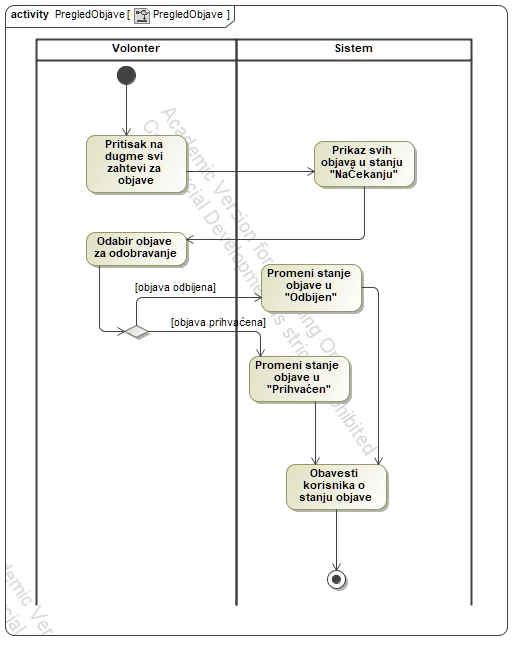
\includegraphics[width=\textwidth, height=\textwidth]{img/activity-post-review.jpg}
    \caption{Dijagram aktivnosti za pregled objave}
    \label{fig:activity-post-review}
\end{figure}


